% Options for packages loaded elsewhere
\PassOptionsToPackage{unicode}{hyperref}
\PassOptionsToPackage{hyphens}{url}
%
\documentclass[
  ignorenonframetext,
]{beamer}
\usepackage{pgfpages}
\setbeamertemplate{caption}[numbered]
\setbeamertemplate{caption label separator}{: }
\setbeamercolor{caption name}{fg=normal text.fg}
\beamertemplatenavigationsymbolsempty
% Prevent slide breaks in the middle of a paragraph
\widowpenalties 1 10000
\raggedbottom
\setbeamertemplate{part page}{
  \centering
  \begin{beamercolorbox}[sep=16pt,center]{part title}
    \usebeamerfont{part title}\insertpart\par
  \end{beamercolorbox}
}
\setbeamertemplate{section page}{
  \centering
  \begin{beamercolorbox}[sep=12pt,center]{part title}
    \usebeamerfont{section title}\insertsection\par
  \end{beamercolorbox}
}
\setbeamertemplate{subsection page}{
  \centering
  \begin{beamercolorbox}[sep=8pt,center]{part title}
    \usebeamerfont{subsection title}\insertsubsection\par
  \end{beamercolorbox}
}
\AtBeginPart{
  \frame{\partpage}
}
\AtBeginSection{
  \ifbibliography
  \else
    \frame{\sectionpage}
  \fi
}
\AtBeginSubsection{
  \frame{\subsectionpage}
}
\usepackage{lmodern}
\usepackage{amssymb,amsmath}
\usepackage{ifxetex,ifluatex}
\ifnum 0\ifxetex 1\fi\ifluatex 1\fi=0 % if pdftex
  \usepackage[T1]{fontenc}
  \usepackage[utf8]{inputenc}
  \usepackage{textcomp} % provide euro and other symbols
\else % if luatex or xetex
  \usepackage{unicode-math}
  \defaultfontfeatures{Scale=MatchLowercase}
  \defaultfontfeatures[\rmfamily]{Ligatures=TeX,Scale=1}
\fi
\usetheme[]{AnnArbor}
% Use upquote if available, for straight quotes in verbatim environments
\IfFileExists{upquote.sty}{\usepackage{upquote}}{}
\IfFileExists{microtype.sty}{% use microtype if available
  \usepackage[]{microtype}
  \UseMicrotypeSet[protrusion]{basicmath} % disable protrusion for tt fonts
}{}
\makeatletter
\@ifundefined{KOMAClassName}{% if non-KOMA class
  \IfFileExists{parskip.sty}{%
    \usepackage{parskip}
  }{% else
    \setlength{\parindent}{0pt}
    \setlength{\parskip}{6pt plus 2pt minus 1pt}}
}{% if KOMA class
  \KOMAoptions{parskip=half}}
\makeatother
\usepackage{xcolor}
\IfFileExists{xurl.sty}{\usepackage{xurl}}{} % add URL line breaks if available
\IfFileExists{bookmark.sty}{\usepackage{bookmark}}{\usepackage{hyperref}}
\hypersetup{
  pdftitle={R install},
  pdfauthor={Эдийн засаг, эконометрикс, статистик},
  hidelinks,
  pdfcreator={LaTeX via pandoc}}
\urlstyle{same} % disable monospaced font for URLs
\newif\ifbibliography
\usepackage{longtable,booktabs}
\usepackage{caption}
% Make caption package work with longtable
\makeatletter
\def\fnum@table{\tablename~\thetable}
\makeatother
\usepackage{graphicx,grffile}
\makeatletter
\def\maxwidth{\ifdim\Gin@nat@width>\linewidth\linewidth\else\Gin@nat@width\fi}
\def\maxheight{\ifdim\Gin@nat@height>\textheight\textheight\else\Gin@nat@height\fi}
\makeatother
% Scale images if necessary, so that they will not overflow the page
% margins by default, and it is still possible to overwrite the defaults
% using explicit options in \includegraphics[width, height, ...]{}
\setkeys{Gin}{width=\maxwidth,height=\maxheight,keepaspectratio}
% Set default figure placement to htbp
\makeatletter
\def\fps@figure{htbp}
\makeatother
\setlength{\emergencystretch}{3em} % prevent overfull lines
\providecommand{\tightlist}{%
  \setlength{\itemsep}{0pt}\setlength{\parskip}{0pt}}
\setcounter{secnumdepth}{-\maxdimen} % remove section numbering
\usepackage[mongolian]{babel}
\usepackage{amssymb,amsmath}
\usepackage[utf8]{inputenc}
\usepackage{graphicx}
\useinnertheme{rectangles}
\titlegraphic{\vfill\includegraphics[height=1.5cm]{econo.png}}

\title{R install}
\author{Эдийн засаг, эконометрикс, статистик}
\date{11/8/2019}

\begin{document}
\frame{\titlepage}

\begin{frame}
  \tableofcontents[hideallsubsections]
\end{frame}
\begin{frame}{WHO AM I}
\protect\hypertarget{who-am-i}{}

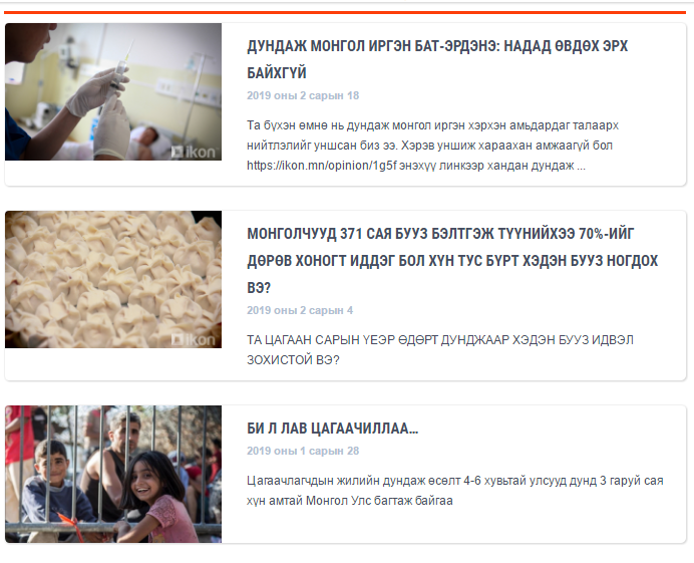
\includegraphics[width=500px]{Picture1}

\begin{itemize}
\tightlist
\item
  { 2008-2012 БАКАЛАВР, МУИС-ЭЗС, ЭДИЙН ЗАСГИЙН ОНОЛ}
\item
  {2015-2018 МАГИСТР, САКАРЯА, ЭКОНОМЕТРИКЧ ЭДИЙН ЗАСАГЧ}
\item
  {ГРАНДЛАЙН БДК, МАКРО ШИНЖЭЭЧ}
\item
  {ХАСБАНК, ЭУГ, ЭРСДЭЛИЙН ШИНЖЭЭЧ}
\item
  {ГОЛОМТ БАНК, ЭУГ, МАКРО ШИНЖЭЭЧ}
\item
  {МБХОЛБООНЫ СУДЛААЧДЫН ЗӨВЛӨЛИЙН ТЭРГҮҮН}
\item
  {IKON.MN -- НИЙТЛЭЛЧ}
\item
  {``ЭДИЙН ЗАСАГЧ'', ``ЭКОНОМЕТРИК СУДАЛЦГААЯ'' АДМИН}
\end{itemize}

\end{frame}

\begin{frame}{WHO AM I}
\protect\hypertarget{who-am-i-1}{}

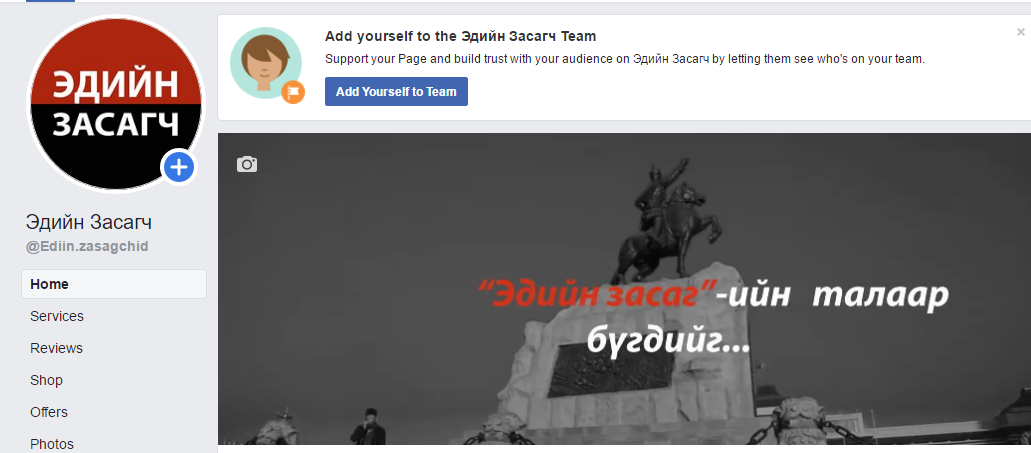
\includegraphics[width=1000px]{Picture2}

\end{frame}

\begin{frame}{Яагаад бид програмын хэл сурах хэрэгтэй вэ?}
\protect\hypertarget{ux44fux430ux433ux430ux430ux434-ux431ux438ux434-ux43fux440ux43eux433ux440ux430ux43cux44bux43d-ux445ux44dux43b-ux441ux443ux440ux430ux445-ux445ux44dux440ux44dux433ux442ux44dux439-ux432ux44d}{}

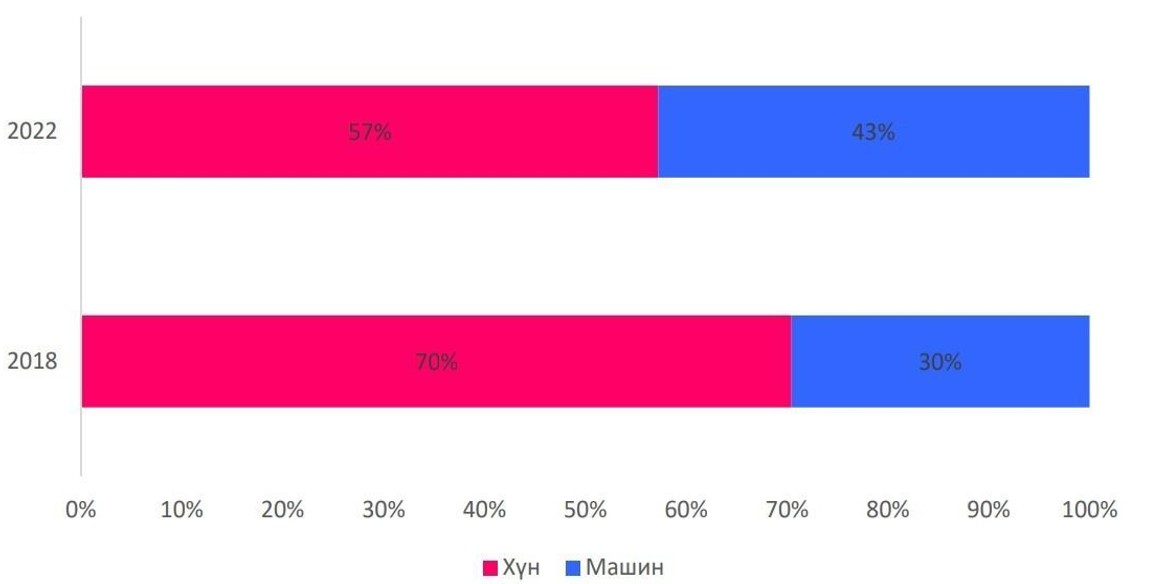
\includegraphics[width=500px]{Picture3}

\begin{itemize}
\item
  Хөгжингүй орнуудаас хөгжиж буй орнууд руу ажилчид шилжинэ.
\item
  Хэрвээ мэргэжилдээ ямар нэгэн диверсифкаци хийхгүй бол машин таныг
  орлох болно.
\end{itemize}

\end{frame}

\begin{frame}{Бид програмын хэл сурвал ямар давуу талтай болох вэ?}
\protect\hypertarget{ux431ux438ux434-ux43fux440ux43eux433ux440ux430ux43cux44bux43d-ux445ux44dux43b-ux441ux443ux440ux432ux430ux43b-ux44fux43cux430ux440-ux434ux430ux432ux443ux443-ux442ux430ux43bux442ux430ux439-ux431ux43eux43bux43eux445-ux432ux44d}{}

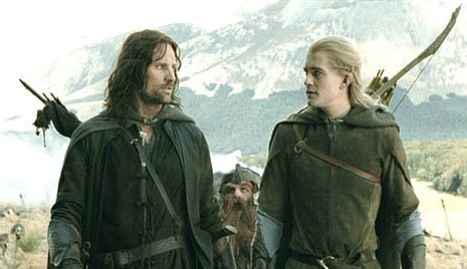
\includegraphics[width=500px]{Picture4}

\begin{itemize}
\tightlist
\item
  Гартаа та хоёр том зэвсэгтэй болно.
\item
  цалингийн хувьд хүссэн цалингаараа ажиллаж чадна.
\item
  одоогийн дата аналистууд бидний салбарыг нарийн ойлгодоггүй.
\item
  ирээдүйд бий болох ажлын байрны хувьд тэсч үлдэх боломжтой.
\item
  одоогоор ирээдүйд ч энэ зүйлс тренд болсоор байна.
\end{itemize}

\end{frame}

\begin{frame}{Top programming language}
\protect\hypertarget{top-programming-language}{}

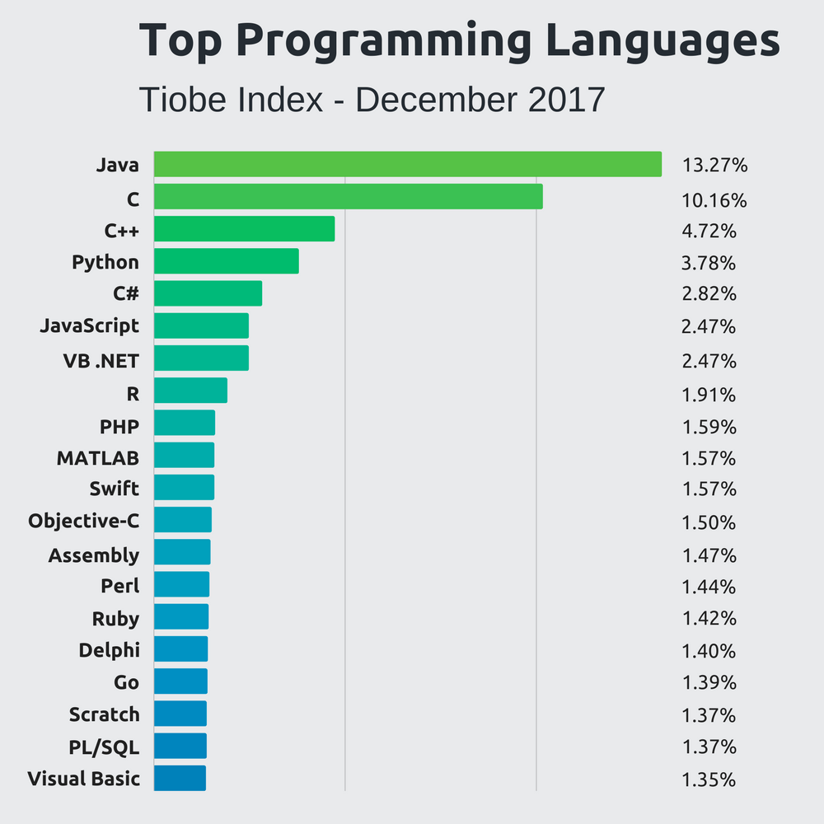
\includegraphics[width=500px]{Picture5}

\begin{longtable}[]{@{}ll@{}}
\toprule
Program names & Salary\tabularnewline
\midrule
\endhead
Python & 166,379\tabularnewline
JavaScript & 110,000\tabularnewline
Java & 97,000\tabularnewline
R & 91,470\tabularnewline
Swift & 81,000\tabularnewline
Golana & 120,000\tabularnewline
C\# & 78,000\tabularnewline
C++ & 116,551\tabularnewline
SCALA & 117,369\tabularnewline
kotlin & 131,250\tabularnewline
\bottomrule
\end{longtable}

\end{frame}

\begin{frame}{WHY IS R Studio}
\protect\hypertarget{why-is-r-studio}{}


\includegraphics[width=400px]{Picture6}


\includegraphics{Capture.JPG}

Ажлын байр болон компани

\begin{itemize}
\tightlist
\item
  Data analyst
\item
  Data scientist
\item
  Financial analyst
\item
  Quantitative analyst
\end{itemize}

\textbf{91,470\$ буюу 240 сая ₮}

\end{frame}

\begin{frame}{What is r studio \{.smaller color:blue .emphasized\}}
\protect\hypertarget{what-is-r-studio-.smaller-colorblue-.emphasized}{}

R хэл нь C++ бичигдсэн.

\begin{itemize}
\tightlist
\item
  статистик тооцоолол
\item
  өгөгдлийн шинжилгээ
\item
  Эконометрикийн шинжилгээ
\item
  Тоон шинжилгээ
\end{itemize}

R хэл нь өгөгдлийн шинжилгээнд (бас machine learning) хамгийн өргөн
ашиглагддаг хэл.

IDE-с гаргасан үнэгүй, нээлттэй шинжилгээний программ юм.

\begin{longtable}[]{@{}ll@{}}
\toprule
\begin{minipage}[b]{0.60\columnwidth}\raggedright
Онцлог\strut
\end{minipage} & \begin{minipage}[b]{0.34\columnwidth}\raggedright
Ашиглалт\strut
\end{minipage}\tabularnewline
\midrule
\endhead
\begin{minipage}[t]{0.60\columnwidth}\raggedright
- Статистик болон дата анализ-д нийтлэг ашигладаг\strut
\end{minipage} & \begin{minipage}[t]{0.34\columnwidth}\raggedright
- Эконометрик загвар, өгөгдлийн шинжилгээ хийх санхүүгийн салбар\strut
\end{minipage}\tabularnewline
\begin{minipage}[t]{0.60\columnwidth}\raggedright
- Нээлттэй, үнэгүй source\strut
\end{minipage} & \begin{minipage}[t]{0.34\columnwidth}\raggedright
- Телекомын салбар\strut
\end{minipage}\tabularnewline
\begin{minipage}[t]{0.60\columnwidth}\raggedright
- Ашиглахад асар их нөөц бололцоотой\strut
\end{minipage} & \begin{minipage}[t]{0.34\columnwidth}\raggedright
- Менежмент\strut
\end{minipage}\tabularnewline
\begin{minipage}[t]{0.60\columnwidth}\raggedright
\strut
\end{minipage} & \begin{minipage}[t]{0.34\columnwidth}\raggedright
- Биологийн салбар\strut
\end{minipage}\tabularnewline
\bottomrule
\end{longtable}

\end{frame}

\begin{frame}{R \& R studio}
\protect\hypertarget{r-r-studio}{}

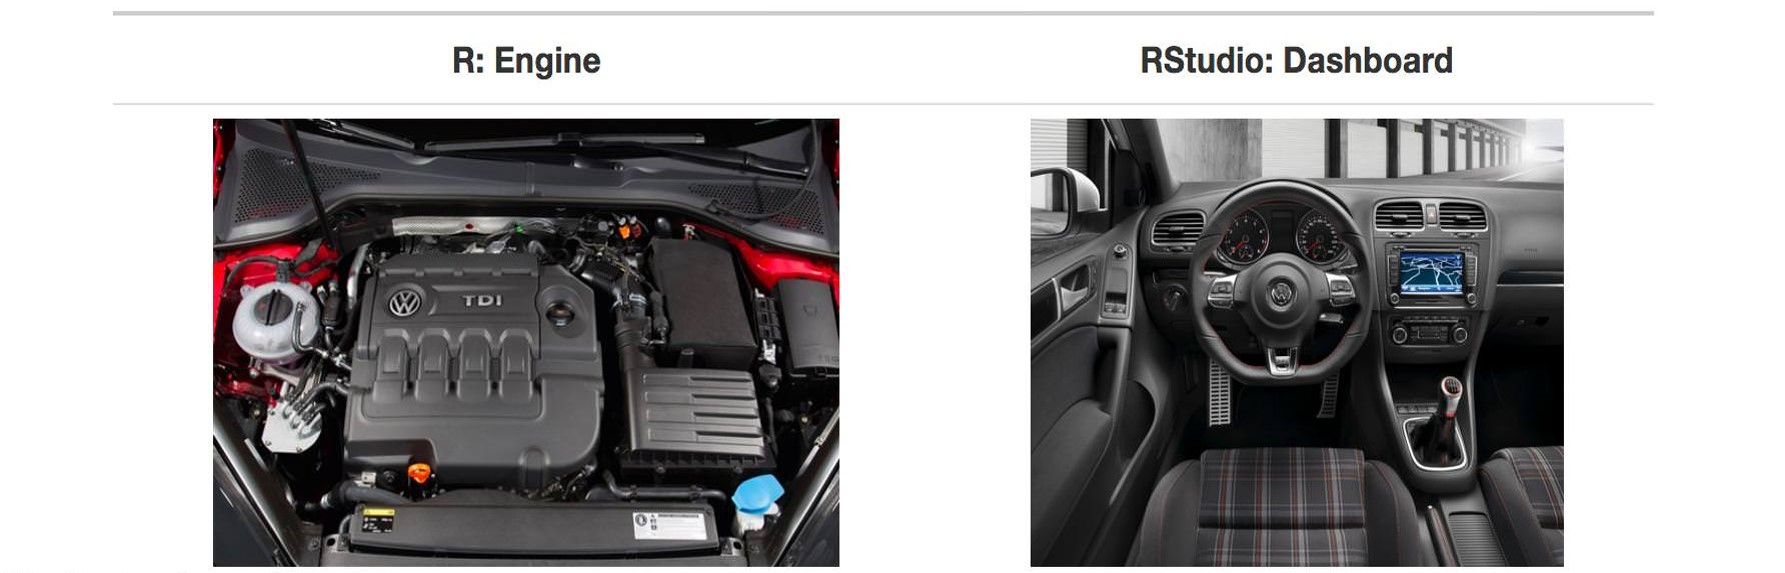
\includegraphics[width=1000px]{Picture7}

\end{frame}

\begin{frame}{R studio installing}
\protect\hypertarget{r-studio-installing}{}

\url{https://www.r-project.org/}

Эхлээд R --г суулгах шаардлагатай. Харин дараа нь Rstudio суулгах
хэрэгтэй.

\url{https://www.rstudio.com/products/rstudio/download/}

Дээрх линкээр орж Windows, Mac, Ubuntu зэрэг аль үйлдлийн систем
хэрэглэж байна. Түүнээсээ хамааран сонгох хэрэгтэй.

Суулгасны дараа цэснүүдтэй танилцах нь

\end{frame}

\begin{frame}{Ажлын цонхтой танилцах}
\protect\hypertarget{ux430ux436ux43bux44bux43d-ux446ux43eux43dux445ux442ux43eux439-ux442ux430ux43dux438ux43bux446ux430ux445}{}

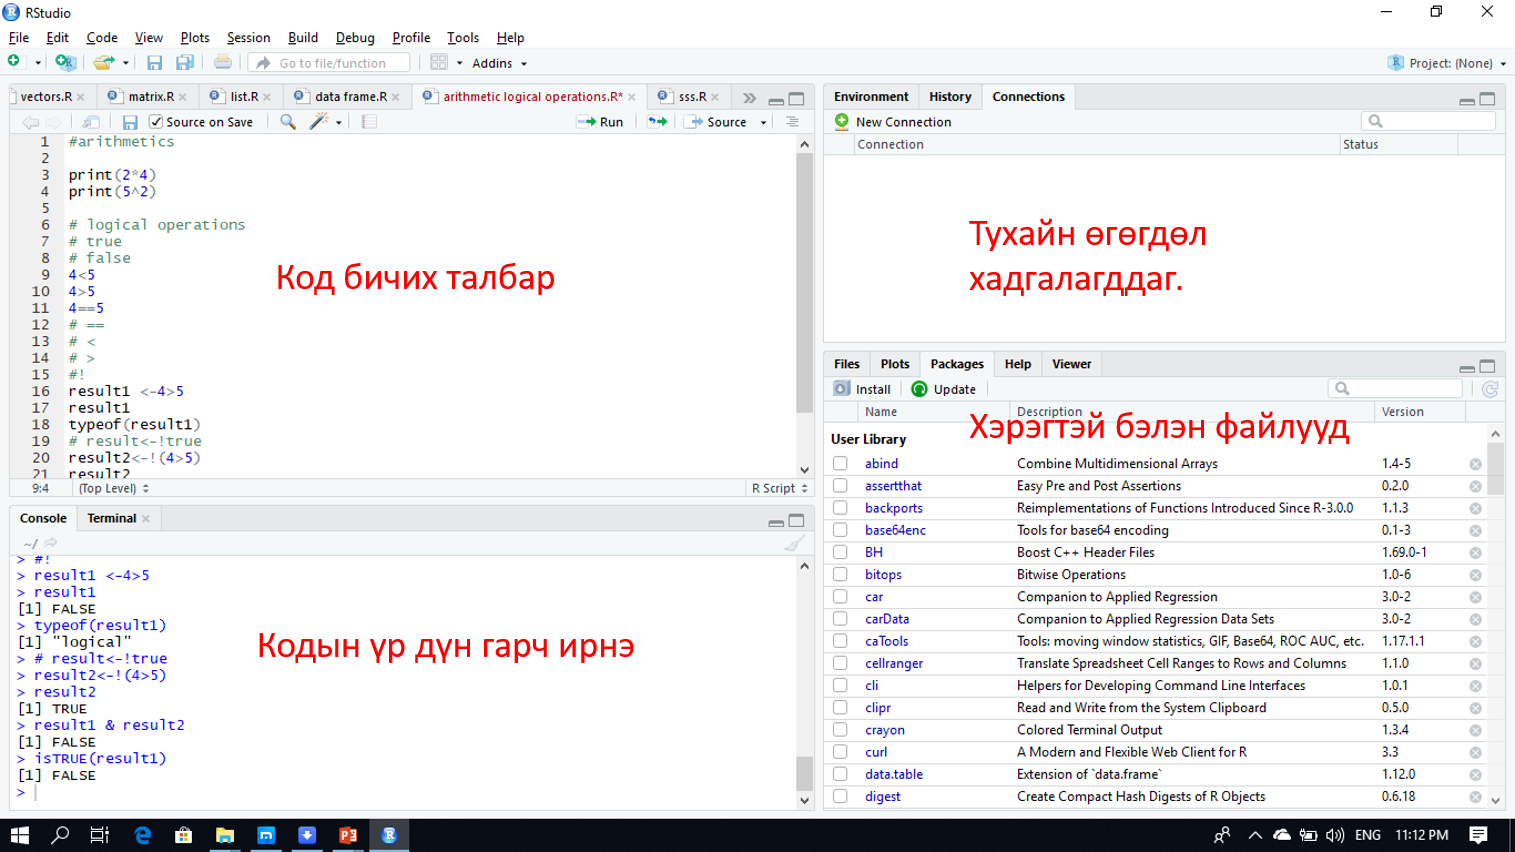
\includegraphics[width=900px]{Picture8}

\end{frame}

\begin{frame}{Анхаарал хандуулсан явдалд баярлалаа}
\protect\hypertarget{ux430ux43dux445ux430ux430ux440ux430ux43b-ux445ux430ux43dux434ux443ux443ux43bux441ux430ux43d-ux44fux432ux434ux430ux43bux434-ux431ux430ux44fux440ux43bux430ux43bux430ux430}{}


\includegraphics{sa.jpg}

\end{frame}

\end{document}
